% =============================================================================
%  封面（Cover）—— 原书封面
%  原书：Brett Slatkin, Effective Python, 3rd Edition (Addison-Wesley)
%  图片取自原版 PDF 第 1 页的整幅封面：images/cover.jpg（1400×1826 px）
%
%  原封面比例 1400:1826 = 0.7667，本书页面 531.36bp × 628.83bp 比例 0.845，
%  两者不同。为了「不拉伸图片」又不留白边，用封面自身的边缘色补边：
%    · 左侧：封面自带的蓝色书脊条（实测 RGB 1,95,156 → #015F9C）
%    · 右侧：封面右缘的深灰底（实测 RGB 36,32,33 → #242021）
%  图片等比缩放到页高（宽 482.11bp）居中，左右各补约 24.6bp 同色，满版出血。
% =============================================================================

% 封面自带的两种边缘色
\definecolor{covSpine}{HTML}{015F9C}
\definecolor{covEdge}{HTML}{242021}

% 图片按 1400:1826 比例撑满页高时的宽度：628.83bp × 0.766703 ≈ 482.11bp
% （先做除法再乘，避免 \dimexpr 中途超过 TeX 的 dimen 上限 16384pt）
\newlength{\covImgW}
\setlength{\covImgW}{\dimexpr\paperheight/1826*1400\relax}

% 图片右缘的横坐标（页面中线 + 半个图宽），右侧深灰底从这条线开始铺
\newlength{\covRightX}
\setlength{\covRightX}{\dimexpr0.5\paperwidth+0.5\covImgW\relax}

\thispagestyle{empty}

\begin{tikzpicture}[remember picture, overlay]
  % 左：蓝色书脊条先铺满整页（图盖住中间后，左侧留下的就是延长后的书脊）
  \fill[covSpine] (current page.north west) rectangle (current page.south east);

  % 右：图片右缘以外补深灰底
  \fill[covEdge]
    ([xshift=\covRightX]current page.north west)
    rectangle (current page.south east);

  % 封面图本体：等比缩放到页高，水平居中
  \node[anchor=center, inner sep=0pt, outer sep=0pt]
    at (current page.center)
    {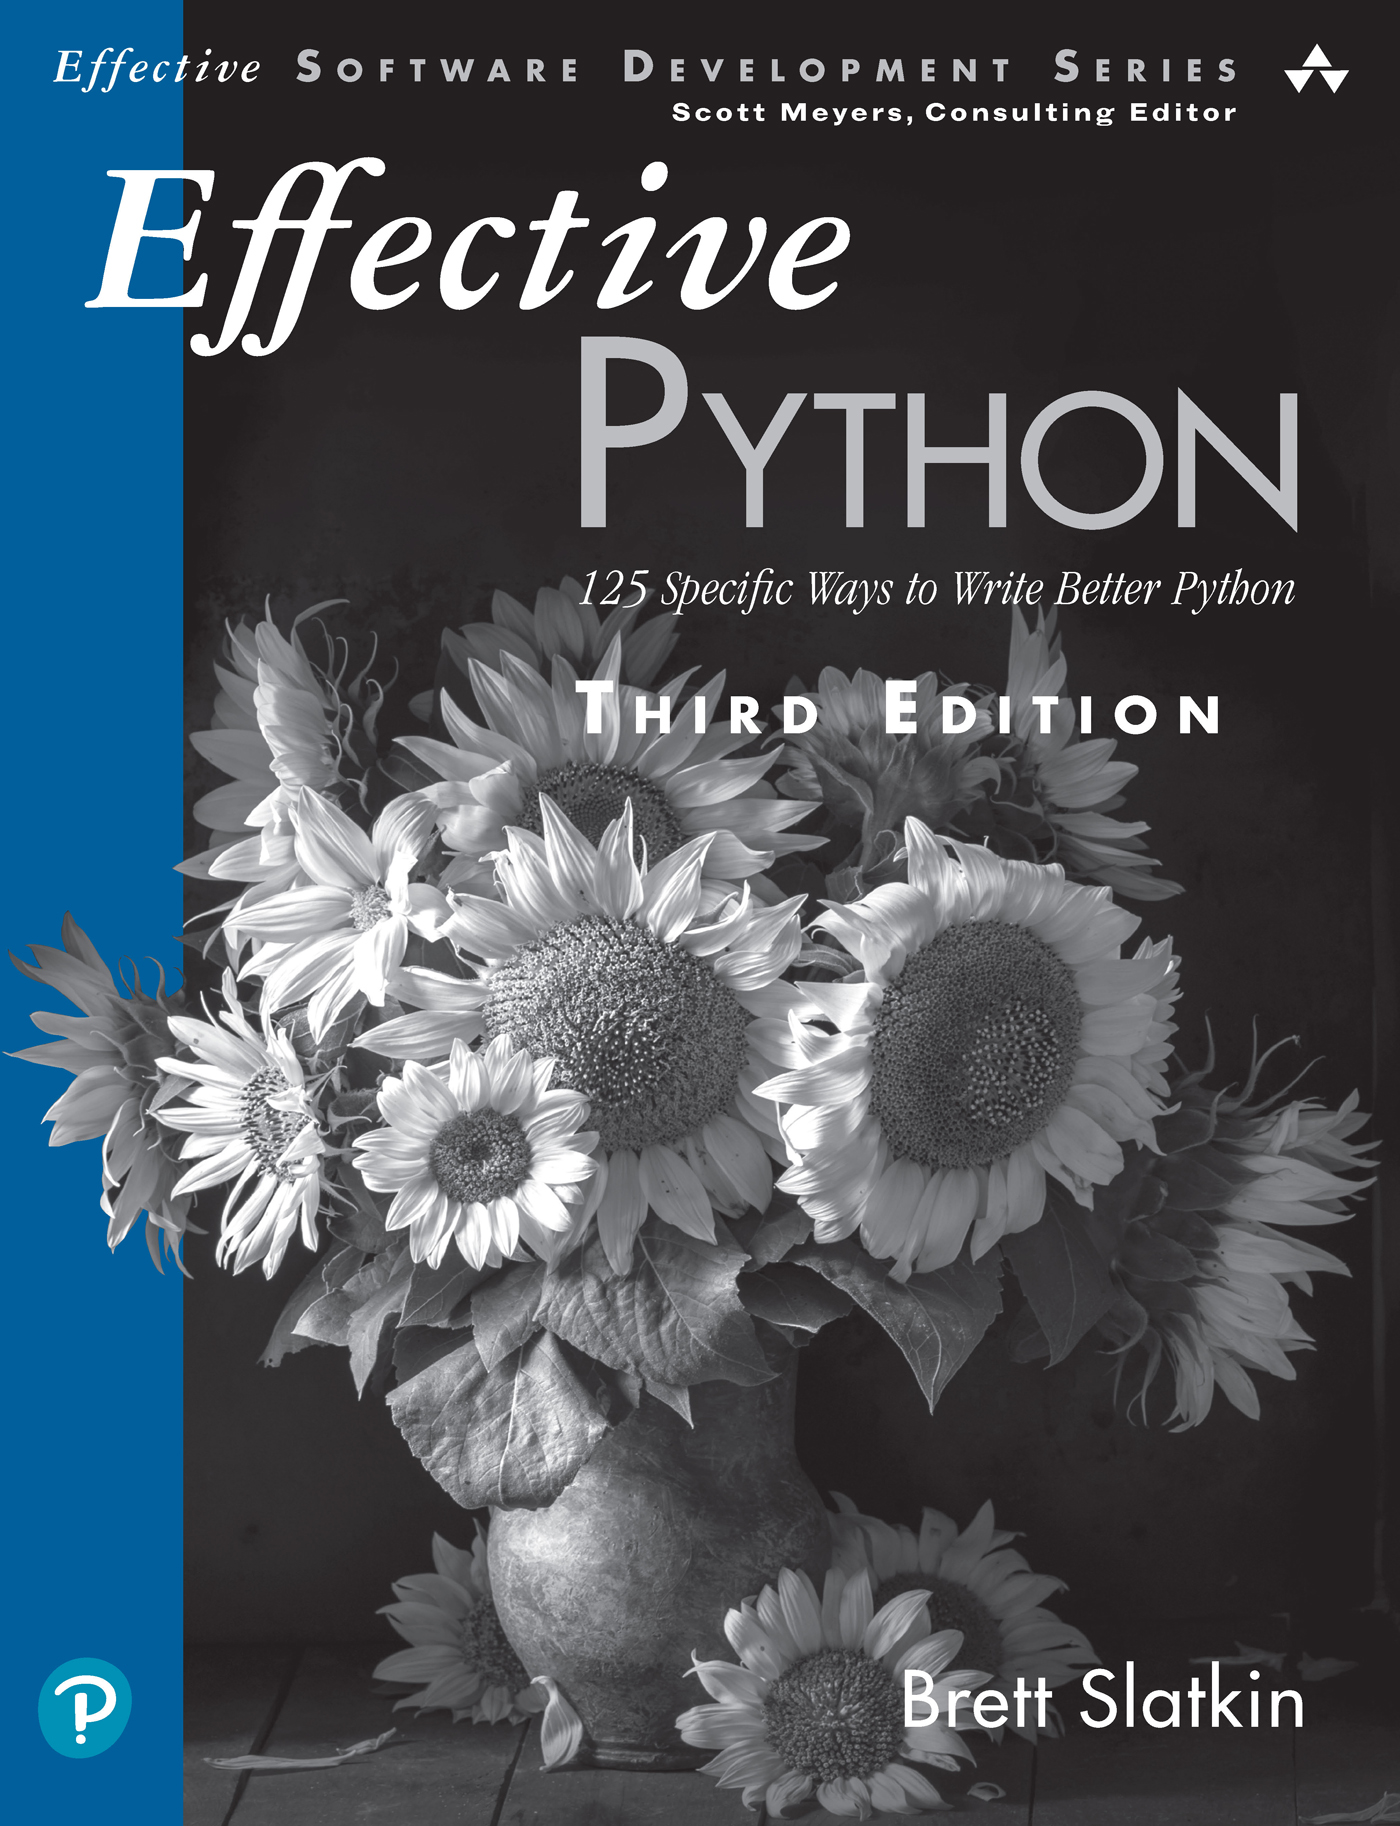
\includegraphics[width=\covImgW, height=\paperheight]{images/cover.jpg}};
\end{tikzpicture}

\null
\clearpage
